\documentclass[10pt,journal,compsoc]{IEEEtran}

\usepackage[nocompress]{cite}
\usepackage{amsmath,amsfonts}
\usepackage{array}
\usepackage{booktabs}
\usepackage{graphicx}
\usepackage{url}
\usepackage{textcomp}
\usepackage{stfloats}
\graphicspath{{../figures/}}

% unnumbered run-in paragraph heading (the class adds the punctuation)
\setcounter{secnumdepth}{3}
\newcommand{\para}[1]{\paragraph{#1}}

\begin{document}

\title{Representations, Generators and Solvers for Perfect 3D Mazes: A Comparative Study}

\author{Mrwan~Alhandi%
\IEEEcompsocitemizethanks{\IEEEcompsocthanksitem M. Alhandi is with the Department of Computer Science.}}

\markboth{CS220 Project Report}{Alhandi: Perfect 3D Mazes: A Comparative Study}

\IEEEtitleabstractindextext{%
\begin{abstract}
Perfect mazes are spanning trees of grid graphs, and they are used in games, puzzles and as testbeds for search algorithms.
Most comparisons of maze algorithms are qualitative and two-dimensional.
We present a reproducible comparative study covering three layers of the problem: the data structure that stores the maze (wall array, adjacency list, adjacency matrix), the generator (recursive backtracking, Prim, Wilson) and the solver (random depth-first search, wall following, Pledge, multi-source breadth-first search), on 2D and multi-level 3D mazes.
We formulate wall following in 3D through a fixed rotation order of the six directions, which keeps its termination guarantee.
We also use a simple solver-aware generator as a stress test.
Across 1440 solver runs, the adjacency matrix's $O(V)$ neighbour queries make it $37\times$ slower than the list for that operation, and it needs $15\times$ the memory at $10^4$ cells.
Generators differ by about $5\times$ in dead-end density and up to $7\times$ in path length, and this reverses the solver ranking: breadth-first search explores the fewest cells on corridor mazes and the most on bushy ones.
The solver-aware generator increases the cells explored by walking solvers by 27--55\%, but not by breadth-first search, which shows that maze difficulty is solver-specific.

\end{abstract}

\begin{IEEEkeywords}
Maze generation, maze solving, spanning trees, graph representations, wall following, comparative study.
\end{IEEEkeywords}}

\maketitle
\IEEEdisplaynontitleabstractindextext
\IEEEpeerreviewmaketitle

% Shared body of the report, included by neurips/main.tex and ieee/main.tex.

\section{Problem Definition}
\label{sec:problem}

A \emph{maze} is a set of cells arranged on a grid in which some pairs of adjacent cells are separated by walls.
We study \emph{perfect} mazes: every cell is reachable from every other cell through exactly one path.
Viewed as a graph whose vertices are cells and whose edges are open passages, a perfect maze is a spanning tree of the grid graph~\cite{buck2015mazes}.
We consider two settings.
In the \emph{2D setting} the grid has $r \times c$ cells.
In the \emph{3D setting} the maze has $L$ levels, where level $\ell$ is an $r_\ell \times c_\ell$ grid; levels may have different sizes, and a cell is also adjacent to the cells directly above and below it when those exist.
Entrances and exits are cells on the outer boundary of a level whose wall to the maze has been removed.

Three problems follow from this definition.
\textbf{(P1) Representation.} The generator and solvers only use two maze operations: setting the wall between two adjacent cells (\texttt{updateWall}) and listing the cells adjacent to a cell (\texttt{neighbours}).
Which data structure (a 2D wall array, an adjacency list or an adjacency matrix) makes these cheap, and what does it cost in memory?
\textbf{(P2) Generation.} Different spanning-tree algorithms produce trees with very different shapes, for example long corridors versus many short dead ends.
How do they differ, and how does the shape affect solving?
\textbf{(P3) Solving.} Given an entrance, a solver walks the maze until it reaches an exit.
Its cost is the number of distinct cells it \emph{explores}.
How do classic solvers compare in 3D?
Two variants complete the problem.
In \emph{best entrance--exit} solving (P3b), the solver may choose the entrance and must find the closest entrance--exit pair while exploring few cells.
In \emph{adversarial generation} (P3c), the generator knows which solver will be used (but may not run it) and must produce a perfect maze that makes that solver explore as many cells as possible.

\section{Literature Review}
\label{sec:literature}

\para{Graph representations}
Adjacency lists use $O(V+E)$ space and enumerate a vertex's neighbours in time proportional to its degree.
Adjacency matrices use $O(V^2)$ space and test an edge in $O(1)$, but enumerating neighbours needs $O(V)$ time~\cite{cormen2009introduction}.
Grid mazes are very sparse ($E < 3V$ in 3D), so textbook analysis predicts that lists dominate.
Maze libraries commonly use an implicit grid array instead, storing one flag per potential wall~\cite{buck2015mazes}.

\para{Maze generation}
Each classic generator is a spanning-tree algorithm.
\emph{Recursive backtracking} is a randomised depth-first search (DFS)~\cite{tarjan1972depth}.
It grows long, winding corridors with few branches.
\emph{Prim's} and \emph{Kruskal's} algorithms build minimum spanning trees~\cite{prim1957shortest,kruskal1956shortest}; with random weights they give bushy mazes with many short dead ends.
The \emph{Aldous--Broder} random walk~\cite{aldous1990random,broder1989generating} and \emph{Wilson's} loop-erased random walk~\cite{wilson1996generating} sample \emph{uniform} spanning trees, so every perfect maze is equally likely.
Wilson's algorithm is the faster of the two.
Pullen~\cite{pullen2023think} and Buck~\cite{buck2015mazes} catalogue these algorithms with qualitative descriptions of their texture (dead ends, river factor, bias).
Kim and Crawfis~\cite{kim2015quest} define quantitative measures of maze difficulty.
Bellot et al.~\cite{bellot2021generate} compare perfect-maze generators statistically.
Maze generation is also a standard technique in procedural content generation for games~\cite{shaker2016procedural}.
Most of these studies are two-dimensional.

\para{Maze solving}
Trémaux's method~\cite{lucas1882recreations} is the historical form of DFS solving.
Breadth-first search~\cite{moore1959shortest} and Dijkstra's algorithm~\cite{dijkstra1959note} return shortest paths, and A*~\cite{hart1968formal} adds a heuristic.
\emph{Wall following} (the left- or right-hand rule) needs no memory and is guaranteed to escape any simply connected maze.
The \emph{Pledge} algorithm~\cite{abelson1980turtle} adds a turn counter so that it can also escape from detached islands when started inside the maze.
Robot ``bug'' algorithms extend this idea to unknown obstacles~\cite{lumelsky1987path}.
Wall following generalises poorly to 3D: there is no global ``left'' once vertical moves exist.
We are not aware of a systematic comparison of these solvers on multi-level mazes, or of how a generator can be tuned against a known solver.

\section{Research Plan}
\label{sec:plan}

We answer four research questions:
\begin{itemize}
  \item \textbf{RQ1} (P1): How do the time per operation and the memory of the three representations scale with maze size?
  \item \textbf{RQ2} (P2): How do recursive backtracking, Prim and Wilson differ in the structure of the 3D mazes they generate?
  \item \textbf{RQ3} (P3, P3b): How many cells do random DFS, wall following, Pledge and multi-source BFS explore, and how does this depend on the generator?
  \item \textbf{RQ4} (P3c): How much can a solver-aware generator increase the cells explored, using only the solver's name?
\end{itemize}

\para{Implementations}
All components share one maze interface, so every generator runs on every representation and every solver runs on every maze.
The \emph{array} stores a $(2r+2)\times(2c+2)$ grid of wall flags.
The \emph{adjacency list} maps each cell to a hash map from neighbour to wall status.
The \emph{adjacency matrix} stores the $V\times V$ matrix, with $V=(r+2)(c+2)$ including boundary cells, as one byte array whose entries encode \emph{no edge}, \emph{open} or \emph{wall}.
\emph{Random DFS} is recursive backtracking with uniformly random choice at junctions.
For \emph{wall following in 3D} we fix one cyclic order of the six directions, (south, west, north, east, up, down).
Arriving from direction $d$, the solver takes the first open direction after $d$ in that order.
For planar moves this is exactly the left-hand rule.
Because every cell uses the same cyclic order (a \emph{rotation system}~\cite{gross1987topological}), the walk is an Euler tour of the passage tree.
It therefore reaches every cell, and hence an exit, in at most $2(V-1)$ moves in any perfect maze.
\emph{Pledge} walks straight in its preferred direction (into the maze), and when blocked follows the wall using the same rule while counting $\pm 90^\circ$ turns.
It resumes walking straight when the counter returns to zero.
Vertical moves leave the counter unchanged.
Pledge's escape guarantee is only proven for planar mazes, so after $4V$ steps the solver falls back to plain wall following.
For best entrance--exit solving (P3b), \emph{multi-source BFS} starts from all entrances at once and stops at the first exit it discovers.
In unit-cost mazes this is equivalent to Dijkstra's algorithm, and that first exit belongs to the closest entrance--exit pair.

\para{Adversarial generator (P3c)}
Any solver must at least walk the unique path from its entrance to the exit it finds.
The generator therefore makes this path long.
It samples $K$ random-DFS spanning trees, with $K=\min(100,\lfloor 2\cdot 10^5/V\rfloor)$, as edge lists without touching the maze, scores each one with BFS on the tree, and carves only the best.
The score depends on the solver's name.
For multi-source BFS it is the shortest entrance--exit distance over all pairs.
For single-entrance solvers, whose entrance is unknown at generation time, it is the mean over entrances of the distance to the nearest exit.

\para{Experimental setup}
\emph{Experiment~1} (RQ1) generates $n\times n$ 2D mazes with recursive backtracking, for $n$ from 10 to 200 (adjacency matrix up to 100, see Section~\ref{sec:results}).
Each size runs with 5 seeds.
We record the generation time, the mean time per \texttt{updateWall}/\texttt{neighbours} call, and the peak memory (\texttt{tracemalloc}) of the initialised maze.
\emph{Experiments~2--4} (RQ2--RQ4) use three 3D settings with two entrances and two exits on different levels:
3 levels of $12\times12$ (432 cells);
3 mixed levels of $10\times10$, $14\times8$ and $8\times14$ (324 cells);
and 4 levels of $20\times20$ (1600 cells).
For each setting and each of 30 seeds, every baseline generator builds one maze that all four solvers solve.
The adversarial generator builds one maze per target solver.
Single-entrance solvers always start from the first entrance.
In total there are 1440 solver runs.
We verify that every generated maze is perfect and that every run reaches an exit.
All experiments ran in Python~3.14 on an Apple M3 Pro with 18\,GB of RAM.
The code and raw results are in the accompanying repository, and the scripts in \texttt{experiments/} reproduce every number in this report.

\section{Contribution}
\label{sec:contribution}

This work is a \textbf{comparative study} (review/survey type).
Its contributions are:
\begin{enumerate}
  \item A unified, reproducible benchmark of three maze representations, three generators and four solvers, extended from the usual 2D setting to multi-level 3D mazes, including levels of different sizes.
  \item A quantitative comparison of generator structure and its effect on solver exploration in 3D.
  It shows that the generator matters as much as the solver.
  \item A 3D formulation of wall following based on a fixed rotation system, which keeps the classical termination guarantee in 3D, together with an empirical check of when Pledge differs from it.
  \item A simple solver-aware generator used as a stress test.
  It measures how far each solver can be pushed and exposes where maximising path length is the wrong objective.
\end{enumerate}

\section{Results}
\label{sec:results}

\begin{figure*}[t]
  \centering
  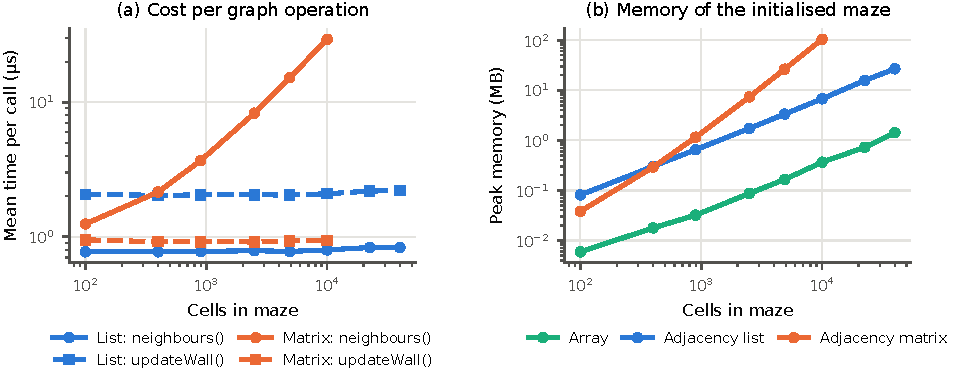
\includegraphics[width=\textwidth]{representations.pdf}
  \caption{Experiment 1 (log--log, mean of 5 seeds). (a) \texttt{neighbours} on the adjacency matrix grows linearly with the number of cells, while the other operations stay constant. (b) The adjacency matrix's memory grows quadratically.}
  \label{fig:representations}
\end{figure*}

\para{RQ1: representations}
Figure~\ref{fig:representations} and Table~\ref{tab:representations} confirm the asymptotic predictions and put sizes on them.
\texttt{updateWall} is constant time in both graphs.
The matrix is about $2\times$ faster per call (0.9 vs.\ 2.1\,$\mu$s) because it indexes a byte array instead of hashing coordinate objects.
\texttt{neighbours}, however, scans a full matrix row.
At $100\times100$ it costs 29.4\,$\mu$s per call, $37\times$ the list's 0.80\,$\mu$s, and the gap grows linearly with $V$.
The generator calls \texttt{neighbours} about $2V$ times, so the matrix's generation time is quadratic (0.67\,s vs.\ 0.14\,s at $100\times100$).
Memory is the binding constraint.
The matrix needs 105\,MB at $100\times100$, $15\times$ the list.
Extrapolating the $O(V^2)$ trend gives about 1.7\,GB at $200\times200$ and 26\,GB at $400\times400$, so we did not run larger matrices.
The array, which encodes only potential walls, is the fastest (0.067\,s) and the smallest (0.37\,MB) by an order of magnitude.
For a fixed grid, implicit adjacency beats either general graph representation.

\begin{table*}[t]
  \centering
  \caption{Experiment 1 at $100\times100$ cells (mean of 5 seeds).}
  \label{tab:representations}
  \small
  \begin{tabular}{lrrrr}
    \toprule
    Structure & Gen.\ (s) & \texttt{updateWall} ($\mu$s) & \texttt{neighbours} ($\mu$s) & Memory (MB) \\
    \midrule
    Array            & 0.067 & --   & --    & 0.37 \\
    Adjacency list   & 0.140 & 2.08 & 0.80  & 6.77 \\
    Adjacency matrix & 0.671 & 0.94 & 29.41 & 104.81 \\
    \bottomrule
  \end{tabular}
\end{table*}

\para{RQ2: generator structure}
Table~\ref{tab:generators} reports structural measures on the largest setting.
The generators produce very different trees from the same grid.
Only 8.7\% of cells in recursive-backtracking mazes are dead ends, compared with 32\% for Wilson and 41\% for Prim.
The entrance-to-exit path is correspondingly long: 324 steps on average, against 81 for Wilson and 47 for Prim.
The share of vertical passages (27\%) barely depends on the generator, which shows that none of them is biased towards or against moving between levels.
Wilson, the only unbiased generator, lies between the two extremes and costs about $2\times$ the time of the others.
The same ordering holds in the two smaller settings.

\begin{table*}[t]
  \centering
  \caption{Maze structure, 4 levels of $20\times20$ (mean of 30 seeds). ``Path'' is the length of the path from entrance~1 to its nearest exit. Adversarial: targeting random DFS.}
  \label{tab:generators}
  \small
  \begin{tabular}{lrrrrr}
    \toprule
    Generator & Dead ends & Junctions & Vertical & Path & Gen.\ (s) \\
    \midrule
    Recursive backtracking & 8.7\%  & 8.6\%  & 26.9\% & 323.8 & 0.045 \\
    Prim                   & 41.4\% & 28.7\% & 27.4\% & 47.3  & 0.048 \\
    Wilson                 & 32.1\% & 25.8\% & 27.7\% & 80.5  & 0.101 \\
    Adversarial (ours)     & 8.7\%  & 8.2\%  & 27.4\% & 858.2 & 1.265 \\
    \bottomrule
  \end{tabular}
\end{table*}

\begin{figure*}[t]
  \centering
  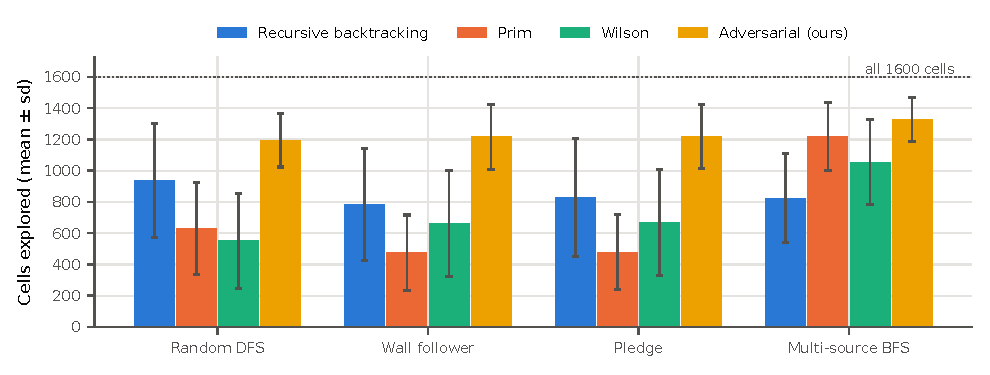
\includegraphics[width=\textwidth]{explored.pdf}
  \caption{Cells explored by each solver on each generator, 4 levels of $20\times20$ (1600 cells, mean $\pm$ sd over 30 seeds). Single-entrance solvers start at entrance~1. Multi-source BFS chooses the entrance itself.}
  \label{fig:explored}
\end{figure*}

\para{RQ3: solvers}
Figure~\ref{fig:explored} shows that the solver ranking depends on the generator.
On Prim and Wilson mazes the three single-entrance solvers explore 30--42\% of the cells, because the exit is close and most dead ends are short.
On recursive-backtracking mazes they explore 49--59\%, because the long path has to be walked in full.
Multi-source BFS shows the opposite trend.
It explores the fewest cells on corridor-like mazes (823, where the frontier is narrow) and the most on bushy ones (1219 on Prim, 76\% of the maze), because the number of cells within a given distance grows with branching.
In exchange it always returns the globally shortest entrance--exit path, and it never backtracks, so its steps equal its explored cells.
DFS, by contrast, takes 1363 steps to explore 936 cells on recursive-backtracking mazes.
Wall following needs no memory, yet it explores fewer cells than random DFS on recursive-backtracking mazes (785 vs.\ 936) and takes fewer steps (1084 vs.\ 1363).
Its deterministic order avoids DFS's random re-entries into side branches.
Pledge differs from wall following only in how it starts.
It explored exactly the same number of cells in 48\% of the runs, and its mean is within 6\% of wall following's in every setting.
This is expected.
Pledge's advantage is escaping islands when starting \emph{inside} a maze, and a perfect maze entered from its boundary has no islands.
The variance is large for all single-entrance solvers (the standard deviation is 40--50\% of the mean): whether the solver happens to commit to the exit's branch early dominates its cost.

\para{RQ4: adversarial generation}
Table~\ref{tab:adversarial} compares the adversarial generator with the strongest baseline for each solver.
Against the three single-entrance solvers it increases the cells explored by 27--55\% in every setting, reaching 74--76\% of the maze.
It also cuts the standard deviation by 41--53\% on the largest setting (Figure~\ref{fig:explored}), because the long path is forced on every run.
Wall following and Pledge gain the most, because their deterministic order cannot shortcut a long path.
Against multi-source BFS the gain is small (+2\% and +9\%) and negative on the mixed-level maze (-11\% versus Prim).
BFS's cost is the number of cells closer than the nearest exit, which depends on branching as much as on distance.
Prim's bushy trees fill that neighbourhood densely, while long DFS corridors do not.
Maximising path length is therefore the right objective for walkers but not for breadth-first searchers.
The price is generation time ($28\times$ recursive backtracking at 1600 cells, because $K=100$ candidates are built), which is affordable offline.

\begin{table*}[t]
  \centering
  \caption{Cells explored: best baseline generator $\rightarrow$ adversarial generator (mean of 30 seeds). R = recursive backtracking, P = Prim.}
  \label{tab:adversarial}
  \small
  \setlength{\tabcolsep}{4pt}
  \begin{tabular}{lccc}
    \toprule
    Solver & $3\times12\times12$ & Mixed 3 levels & $4\times20\times20$ \\
    \midrule
    Random DFS       & R 255 $\rightarrow$ 323 (+27\%) & R 168 $\rightarrow$ 222 (+32\%) & R 936 $\rightarrow$ 1194 (+28\%) \\
    Wall follower    & R 230 $\rightarrow$ 321 (+39\%) & R 160 $\rightarrow$ 226 (+41\%) & R 785 $\rightarrow$ 1216 (+55\%) \\
    Pledge           & R 225 $\rightarrow$ 324 (+44\%) & R 164 $\rightarrow$ 230 (+40\%) & R 826 $\rightarrow$ 1220 (+48\%) \\
    Multi-source BFS & P 348 $\rightarrow$ 355 (+2\%)  & P 276 $\rightarrow$ 246 (-11\%) & P 1219 $\rightarrow$ 1325 (+9\%) \\
    \bottomrule
  \end{tabular}
\end{table*}

\section{Conclusion and Discussion}
\label{sec:conclusion}

We compared maze representations, generators and solvers on 2D and multi-level 3D perfect mazes.
Four conclusions emerge.
(i) For grid mazes, an implicit wall array beats both general graph representations.
Between those two, the adjacency list is the practical choice: the matrix's per-call \texttt{updateWall} advantage is outweighed by $O(V)$ neighbour queries and $O(V^2)$ memory, which already reaches 105\,MB at $10^4$ cells.
(ii) The generator decides the maze's character: recursive-backtracking mazes have about $5\times$ fewer dead ends and paths up to $7\times$ longer than Prim's.
It also decides which solver looks best, so solver comparisons on a single generator are misleading.
(iii) In 3D, wall following stays complete under a fixed rotation order of the six directions, and it is competitive with random DFS while using no memory.
Pledge adds nothing in perfect mazes entered from the boundary.
Multi-source BFS is the right tool when the shortest pair matters, but its exploration cost depends heavily on branching.
(iv) A generator that knows only the solver's name can raise the exploration of walking solvers by 27--55\%.
The same objective fails against breadth-first search, so adversarial generation needs a solver-specific notion of difficulty.

\para{Limitations and future work}
Timings come from Python, where interpreter overhead compresses constant factors; the asymptotic trends, not the absolute numbers, are the transferable result.
The 3D settings are moderate (at most 1600 cells), and each single-entrance solver always starts from the same entrance.
The adversarial generator searches only over DFS trees.
For BFS-like solvers a natural next step is to search directly for trees that maximise the number of cells within the entrance--exit radius, for example by local search over spanning trees or with uniform sampling~\cite{wilson1996generating} as a proposal distribution.
Extending the difficulty measures of Kim and Crawfis~\cite{kim2015quest} to multi-level mazes is another open direction.


\bibliographystyle{IEEEtran}
\bibliography{../references}

\end{document}
